
\graphicspath{ {mainmatter/Overholt_2005/} }
\title*{2005: The Overtone Violin}
\titlerunning{The Overtone Violin}

\author{Dan Overholt}
\authorrunning{Overholt}

%\institute {Dan Overholt \at Aalborg University Copenhagen, Denmark, At the date of original
%publication, the author was doubly affiliated with CREATE: Center for Research in
%Electronic Art Technology at U.C. Santa Barbara, and STEIM: Studio for
%Electro-Instrumental Music in Amsterdam, The Netherlands., \email{dano@create.aau.dk}}
%
%
\maketitle

\abstract*{This paper describes the concept, design, realization and evaluation of a
radically augmented musical instrument named the Overtone Violin. The rationale
behind the development of the instrument is to preserve the expressive elements
of the expert violinist, while incorporating the added benefits of gestural
controllers via embedded sensors. There have been many examples of idiosyncratic
alternate controllers in electronic music, as well as quite a few hybrid
controllers that typically use sensors to capture the motions of playing a
traditional instrument. However the Overtone Violin crosses these boundaries by
retaining the original violin techniques and sounds as well as
extending/enhancing the instrument with new methods of expression that are not
inherent to the conventional technique.}

\section{Introduction}

The pursuit of novel interfaces for new music performance is a very interesting
angle from which to approach the design of a musical instrument, but without the
proper perspective the result can be hard to differentiate between a musically
useful device and a simple gadget. There is of course the typical industry
approach of building electronic instruments in the likeness of an existing
(acoustic) instrument, and while this can be useful, such imitation lacks the
creative effort that can lead to new innovations. However, ignoring the
background and not building on an existing tradition can be hazardous as well, as
it can either be too far ahead of its time or end up being merely a gimmick.
Although the evolution of most acoustic instruments has stagnated, there are
recent examples of hybrid instruments \cite{Bongers:1994,Burtner:1994,Machover:1992a} that augment traditional
instruments with additional gestural capabilities. The Overtone Violin fits into
this category.

Any instrument can be augmented to different degrees through the addition of
extra sensors. Hybrid instruments offer musicians the familiarity and
expressivity of their chosen instrument along with the extended control afforded
by the sensors. There are two ways, however, in which the Overtone Violin differs
from most hybrid instruments. First, the extra sensors are used to capture a new,
separate set of gestures; many hybrid instruments use sensors just to acquire
techniques that are part of the traditional skills of the performer. And second,
it is custom designed and built from scratch to be an entirely new, specialized
instrument that continues the evolution of the violin (rather than adapting or
retrofitting an existing instrument with some sensors tacked on). The philosophy
behind this approach is to use gesture sensors to add completely different
functionality to the instrument rather than capturing playing techniques that
already have their own outcome---in this case, the sound of the strings. In fact,
the Overtone Violin can be viewed as two components tightly integrated into one:
it is both a traditional (electro-acoustic) violin, and a gestural computer music
controller.

\begin{figure}[t]
\centering
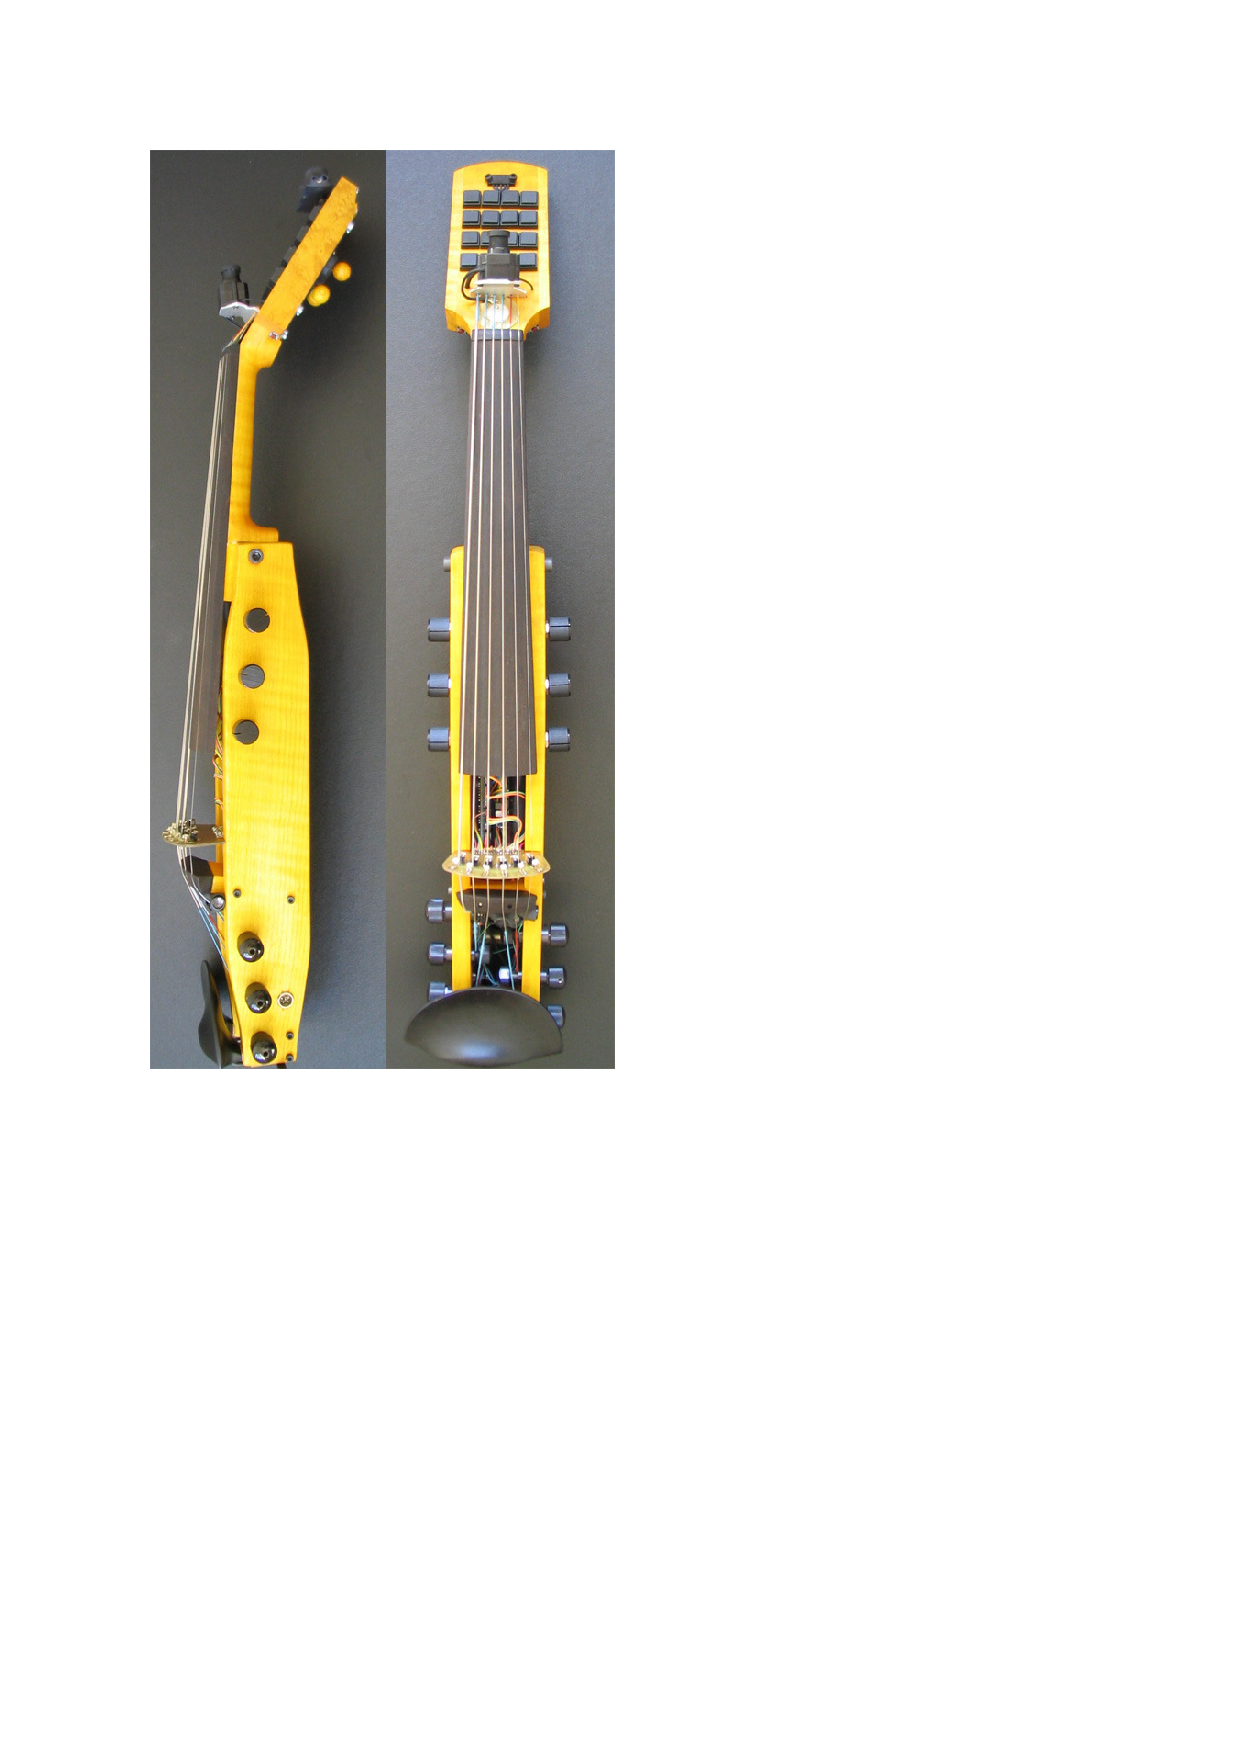
\includegraphics[width=222pt]{img-1-eps-converted-to.pdf}
\caption{The Overtone Violin.}
\label{Overholt:fig:1} 
\end{figure}

As can be seen in Figure~\ref{Overholt:fig:1}, the violin itself is improved though the addition of
extra strings (six strings instead of four, extended downwards into the cello
range) and the tuning machines are located at the bottom in order to allow
gesture sensors to be placed at the head of the instrument. A custom optical
pickup system provides independent audio signals from each string, plus there is
a monophonic audio output using a standard $1/4^{\prime\prime}$ guitar jack.
Details of the optical audio pickups and sensor electronics implementation are
included in sections 3.1 and 3.2 respectively.

\section{Motivation and Background}

One of the primary motivations behind the Overtone Violin is to put real-time
signal processing under direct expressive control of the performer, thereby
pushing the envelope of violin performance and composition into completely new
areas. Through the combination of violin performance technique and gestural
control, employing a virtually unlimited number of synthesis possibilities and
mapping strategies, the Overtone Violin can be used for a wide range of musical
purposes.

Trained violinists are able to pick up the Overtone Violin and play the strings
fluently. However, there is another gesture vocabulary beyond that of acoustic
violins in dealing with the extra sensors that requires the development of new
skills to master. While this necessitates new playing techniques, the process of
learning is facilitated by similarities to the older technique. For example, the
16-button matrix at the head of the instrument is fingered with the left hand, as
are the violin strings themselves. It is by design that there is no direct
overlap between the two types of instrument manipulations, because if they were
synonymous the instrument would be incapable of controlling new sounds
independently. For instance, using sensors to obtain gesture data from
established violin technique may be interesting from a strictly engineering or
pedagogical point of view, but the artist who wishes to have technology do more
than reflect their old gestures should expect to spend time learning a new
vocabulary just as they spent years practicing traditional technique.

However, there are countless possibilities for using signal processing to
mirror/modify the string sounds from the Overtone Violin---in fact the
independent audio signals from each string are intended to help in this process
by providing clean signals for pitch detection/feature tracking, and allowing
different algorithms/spatializations to be applied to each string. Signal
processing is a very powerful way to enhance the violin without having to learn a
new gesture vocabulary \cite{Jehan:2001b,Poepel:2004}, as it preserves the nuances and subtleties of a
skilled performer. But traditional instrumental techniques are not well suited
for the parametric control of signal processing (e.g., audio effects or synthesis
algorithms), so gestural controllers are needed as well. The Overtone Violin is a
powerful research tool to investigate innovative approaches to combining signal
processing of traditional violin sounds with gestural control.

There are many people who have worked on augmenting the violin in different
ways, some of whom have directed their efforts exclusively towards signal
processing \cite{Jehan:2001b,Poepel:2004,Serafin:1999}, and others who focus more on the input device (a classic
example is Max Mathew's Violin \cite{Mathews:1984}, which used piezoceramic bimorph pickups with
resonant equalization). However, there have only been a few true hybrid bowed
string instruments that incorporate gesture sensors with traditional technique.
Chris Chafe developed his Celleto \cite{Chadabe:1997} and has used accelerometers and the Buchla
Lightning IR tracker to measure the dynamics of the bow. Camille Goudeseune
measures violin position and orientation using a SpacePad motion tracker and the
relative position of the bow and violin with magnetic sensors \cite{Goudeseune:2001}. Some
instruments though are actually alternate controllers which were only inspired by
the violin, such as Dan Trueman's BoSSA \cite{Trueman:1999}, Suguru Goto's Super-Polm \cite{Pierrot:1997}, and
Charles Nichol's vBow \cite{Nichols:2003}. These keep some violinistic traditions but do not
have real strings, and drop genuine violin technique entirely in favor of
analogous control methods. Peter Beyls IR-violin \cite{Cutler:2000} also fits into this category
even though it is built into a conventional acoustic violin. Related also are the
Hyperbow by Diana Young \cite{Young:2002}, and Jon Rose's MIDI bow.\footnote{\url{http://www.jonroseweb.com}}

\section{Design of the Overtone Violin}

The development of the Overtone Violin was a complicated process, and involved
quite a few different disciplines. One of the first decisions encountered was the
choice of material to use for the construction. While this one uses curly violin
maple, the design could be built using many different woods or other less
traditional materials. The neck and body were hand carved and machined using a
milling machine. While it is possible to purchase pre-made violin fingerboards,
the use of six strings called for a wider fingerboard, so a viola fingerboard was
used with the extra length removed from the narrow end. The electronics in the
Overtone Violin are powered by a 10-Volt rechargeable NiMH battery pack located
in between the two ribs along with all of the circuit boards and wiring. A
trickle-charging circuit is built in, and there is a DC-input jack on the left
side of the body---the violin can be used while charging, or the battery will
last 3-4 hours with everything powered on.

\subsection{Optical Audio Pickup}

The pickup system used on the Overtone Violin is an adaptation of an electric
bass/guitar pickup made by Lightwave Systems.\footnote{\url{http://lightwave-systems.com/}}

\begin{figure}[t]
\centering
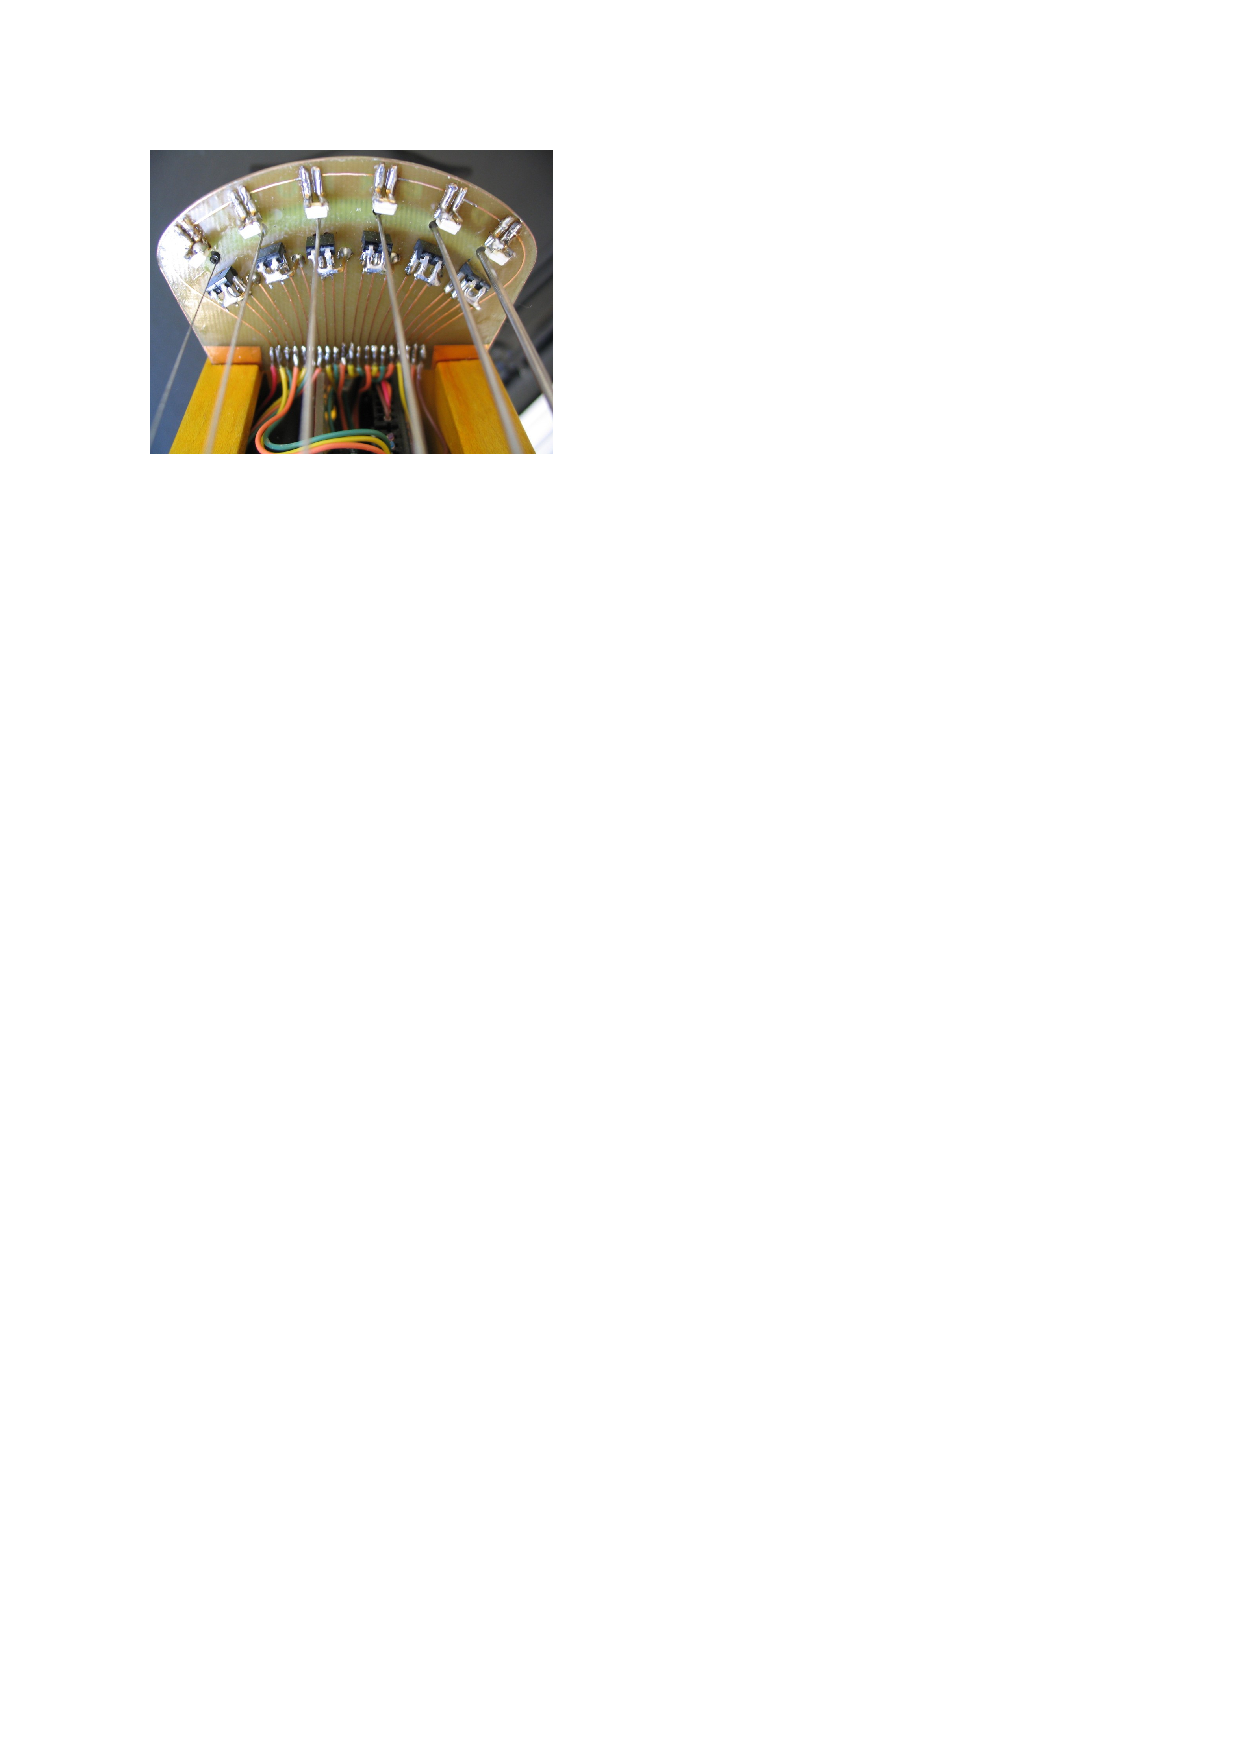
\includegraphics[width=193pt]{img-2-eps-converted-to.pdf}\textbf{ }
\caption{Overtone Violin bridge/PCB with optical pickups.}
\label{Overholt:fig:2} 
\end{figure}

As seen in Figure~\ref{Overholt:fig:2}, there are six IR LEDs above the strings, and a pair of IR
photodiodes below each string. These are mounted on a custom circuit board that
doubles as the violin's bridge. In this manner, infrared light is directed across
each string in order to cast a moving shadow on the photodiodes. The instrument
does not need a resonating body, as the optics sense the string's vibrations
directly and very precisely through differential occlusion, and the resulting
sound is quite good.\footnote{Tone is a matter of personal preference, but the
author is quite pleased with the timbre quality of the optical pickup system.}

The optical pickup system was developed in an attempt to improve the quality of
sound as compared to other violin pickup systems, and is unique to the author's
knowledge. The bridge circuit board is made from a sheet of epoxy fiberglass
laminate using the common process of developing and etching PCBs. Making the
bridge this way allows for optimal placement of the pickup optics, and minimizes
interference with bowing techniques such as ``sul ponticello'' (near the bridge).
But because there is no easy way to modify the height of the bridge (conventional
violin makers simply shave wood from the bridge to adjust the action of the
strings), the angle between the neck and the body of the instrument is adjustable
using a set screw underneath the instrument. In this way, the height of the
strings above the fingerboard can be changed.

A monophonic audio output is provided on the left side of the instrument, and a
13-pin DIN connector with individual string outputs is available as well on the
underside of the violin, following the standard pinout used by Roland on their
Virtual Guitar (VG-8 series) and MIDI guitar converters. The Overtone Violin can
be plugged directly into either of these, or used with a commercial breakout box
to get access to the string signals independently. The three rotary
potentiometers on the left side of the body of the instrument are connected to
the Lightwave active electronic pre-amplifier, and control volume, tone, and
``MIDI-volume'' (used with Roland gear) respectively.

\subsection{Gesture Sensors}

The sensor system on the Overtone Violin includes 18 buttons, 3 rotary
potentiometers, 2 linear potentiometers, 1 spring-loaded slider-type
potentiometer, 1 miniature joystick x/y, a 2D accelerometer x/y, 2 channels of
sonar (one in direct and one in echo mode), and a miniature video camera. The
majority of these sensors are located on both sides of the head of the violin
(see Figure~\ref{Overholt:fig:3}).

\begin{figure}[t]
\centering
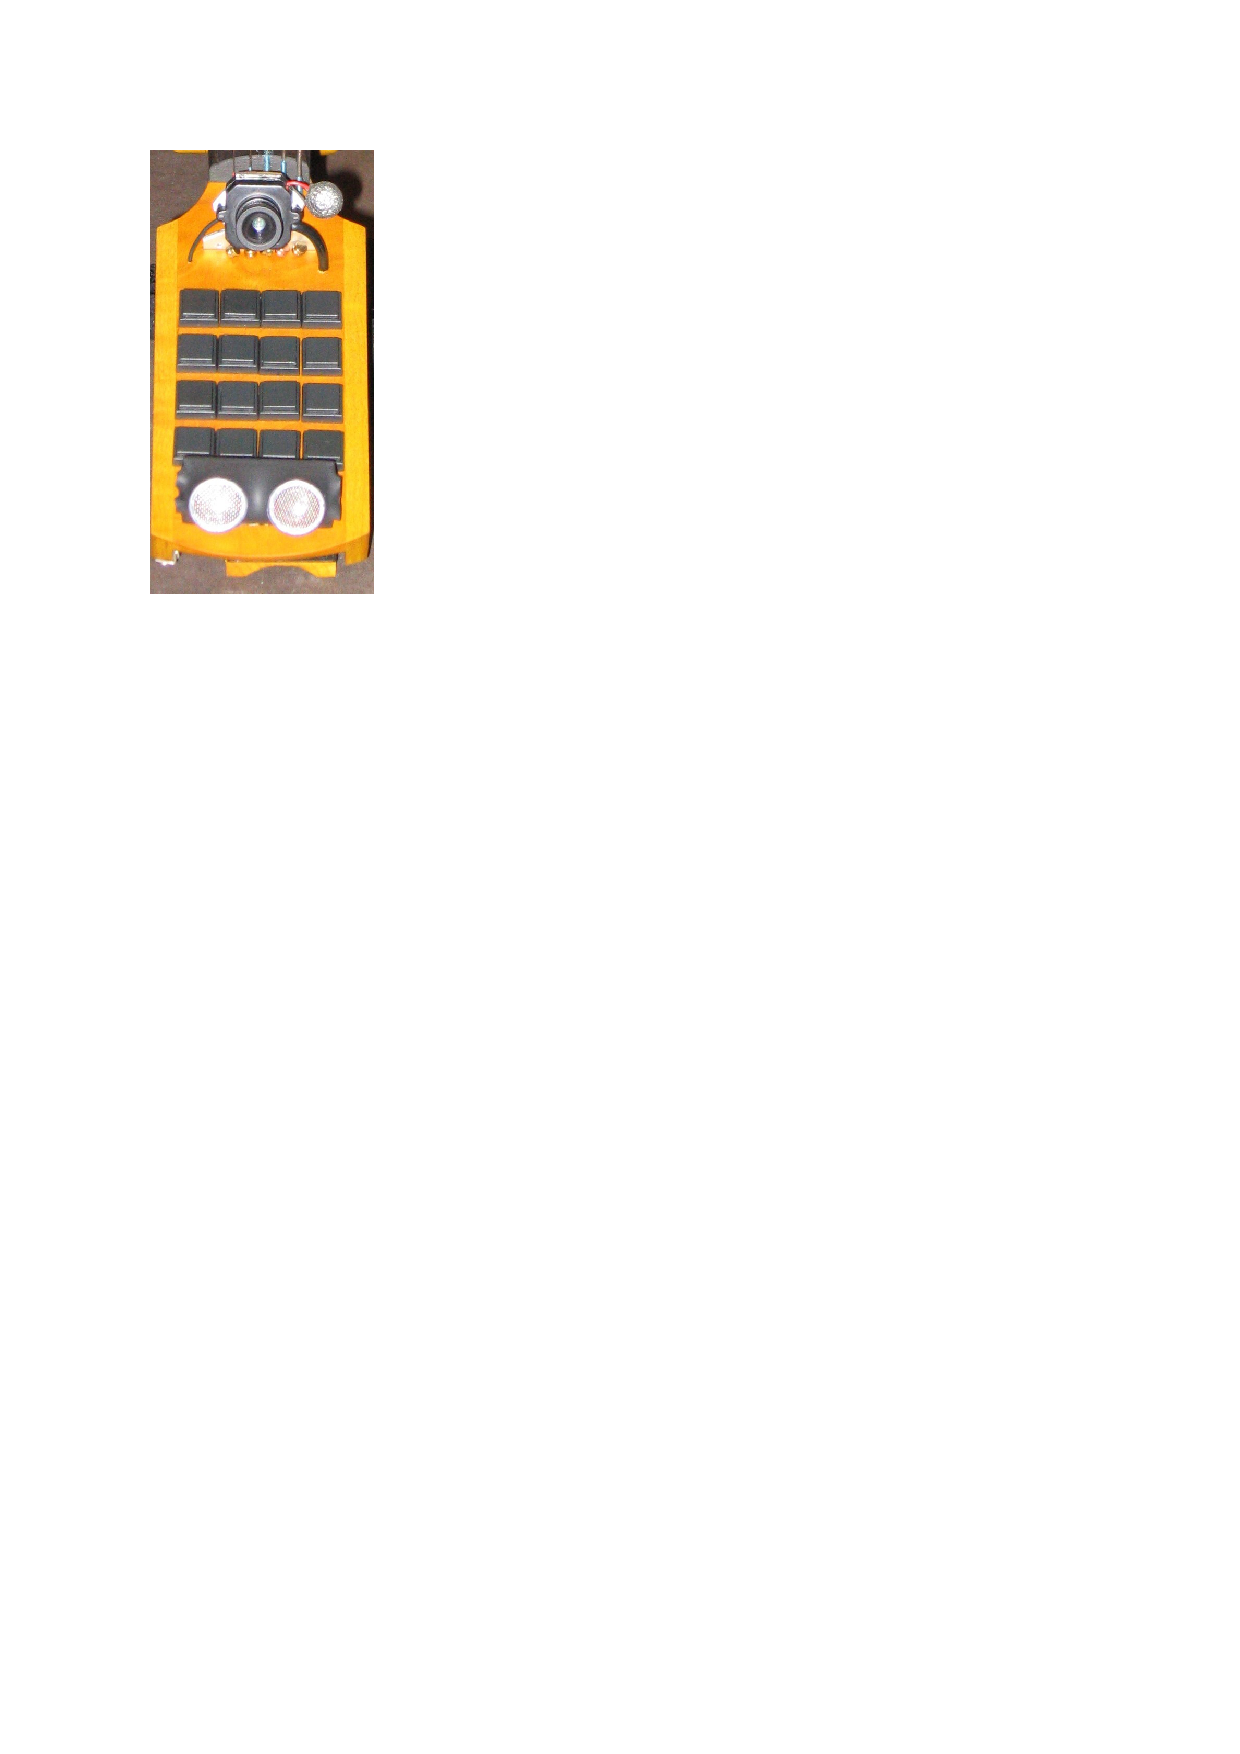
\includegraphics[width=108pt]{img-3-eps-converted-to.pdf}  
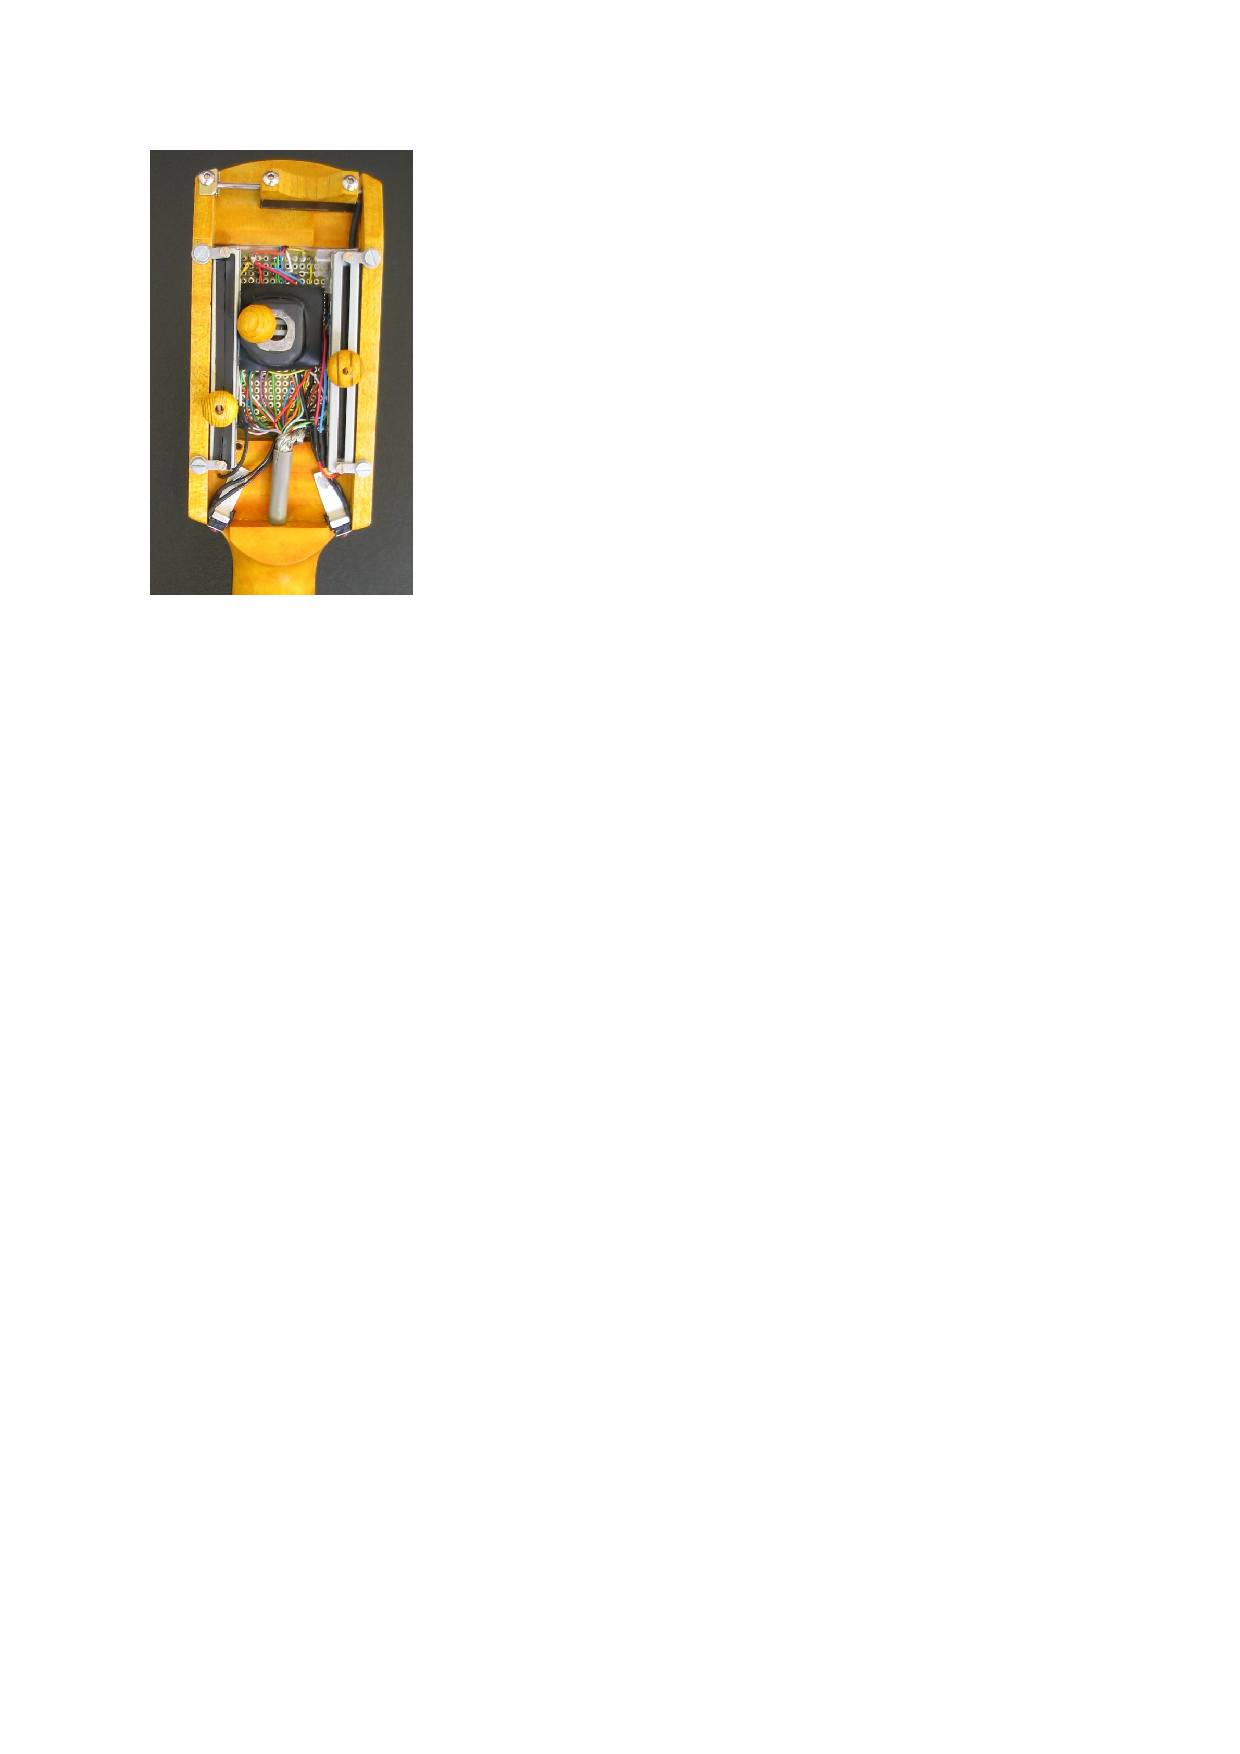
\includegraphics[width=126pt]{img-4-eps-converted-to.pdf}
\caption{Sensors on the head of the Overtone Violin.}
\label{Overholt:fig:3} 
\end{figure}

There is a channel inside the violin's neck for the sensor wires to run through
in order to connect to a microcontroller (Microchip PIC16F877) located in the
body of the violin. This PIC converts all of the analog and digital sensor values
to a serial stream that is sent to an RF transmitter also in the body of the
violin (Radiometrix TX2-433). With this wireless link, a performer can walk onto
the stage just as an acoustic violinist does---all the electronics can be left
off-stage. The miniature video camera also has it's own built-in RF transmitter,
and the audio from the violin strings can be transmitted to the computer for
signal processing via a commercial wireless guitar system.

The sensor data is received through a USB-powered RF receiver (see Figure~\ref{Overholt:fig:4})
that uses another microcontroller (Microchip PIC16C745) to translate the RF data
into USB. For ease of use, the sensor data is translated into the USB standard
protocol for game controllers (the firmware of the PIC enumerates as a
multi-axis, multi-button game controller with the device name ``Overtone
Violin''). This makes the task of communicating with software such as
SuperCollider, Max/MSP/Jitter, Pd, etc. much simpler, because these programs
already have built-in support for game controllers through the HID (Human
Interface Device) drivers. The use of USB has several advantages over MIDI, such
as lower latency, bus-power (no need for batteries or a power adapter), and
simply not having to carry around a MIDI interface.

\begin{figure}[t]
\centering
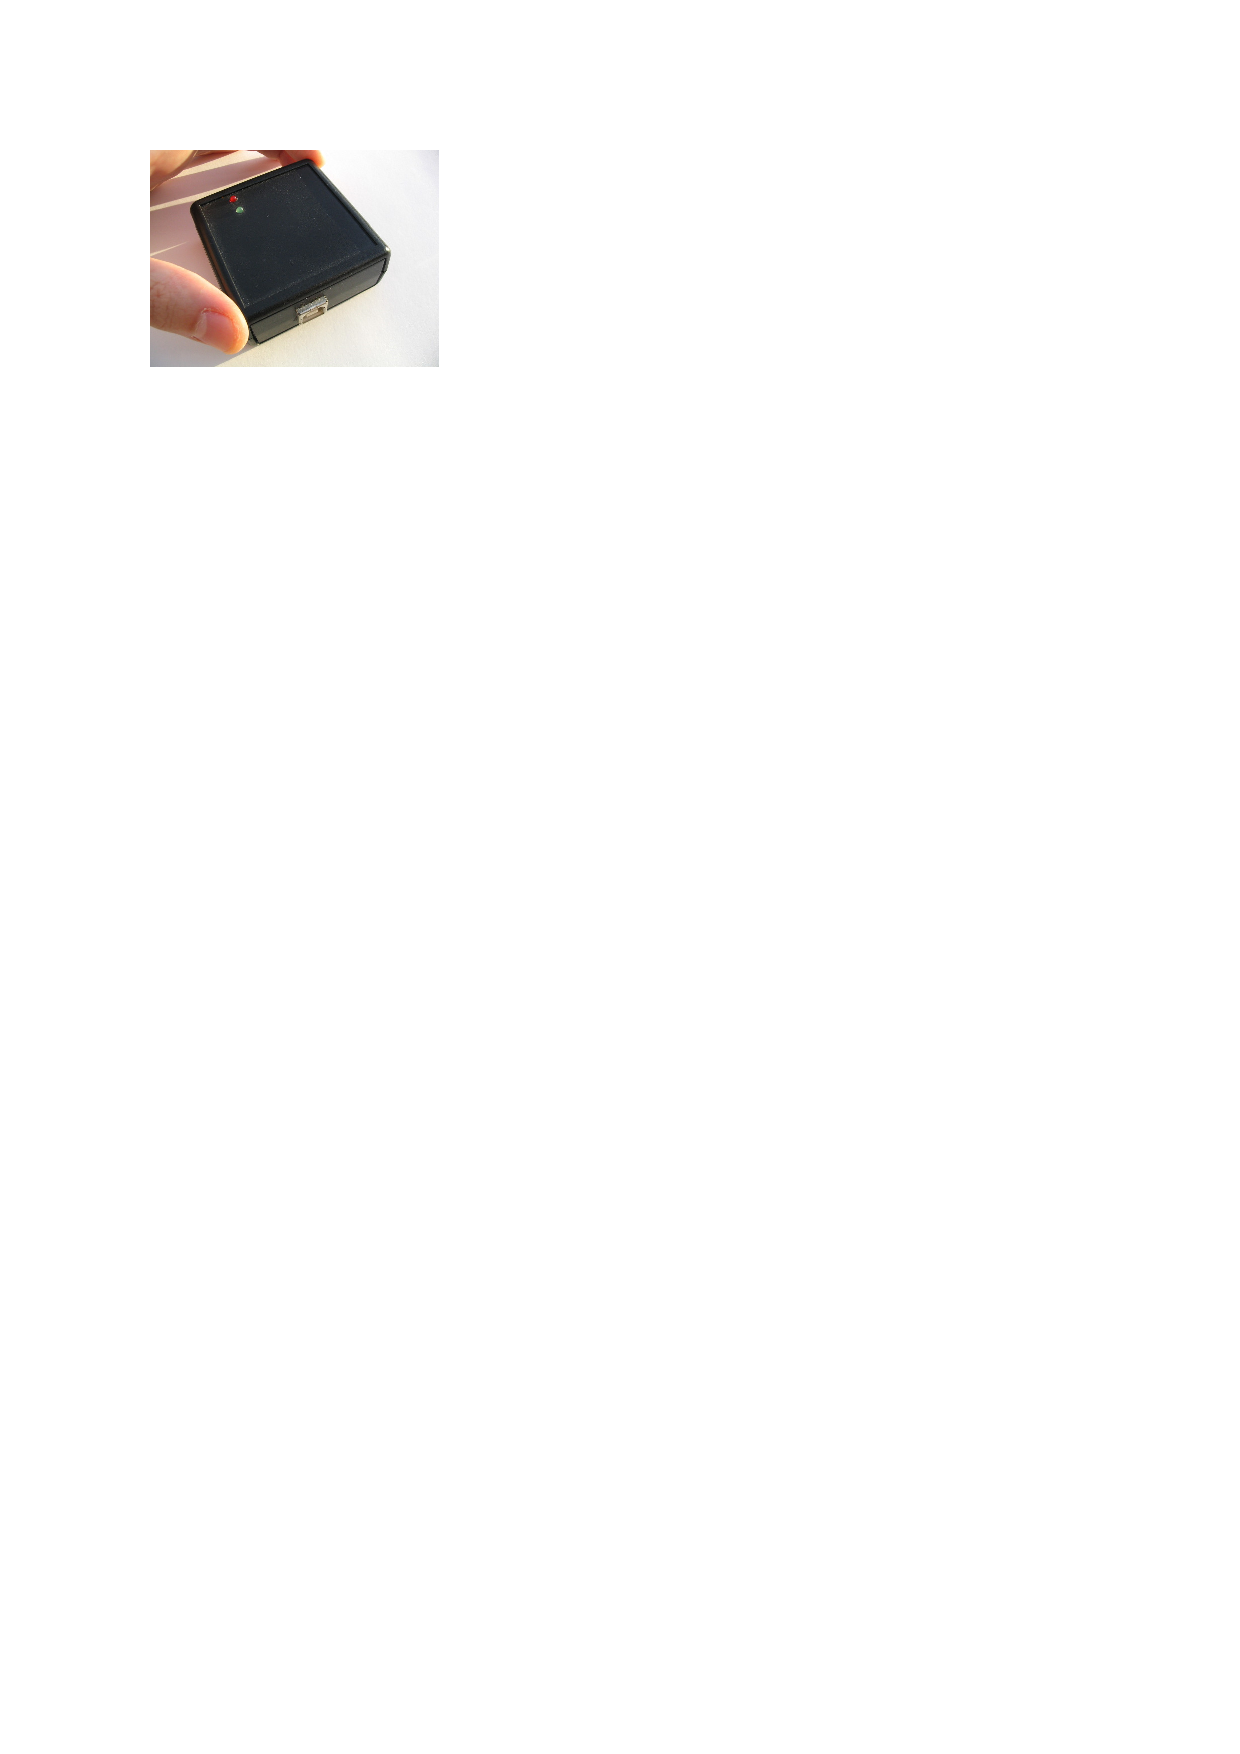
\includegraphics[height=45mm]{img-5-eps-converted-to.pdf}
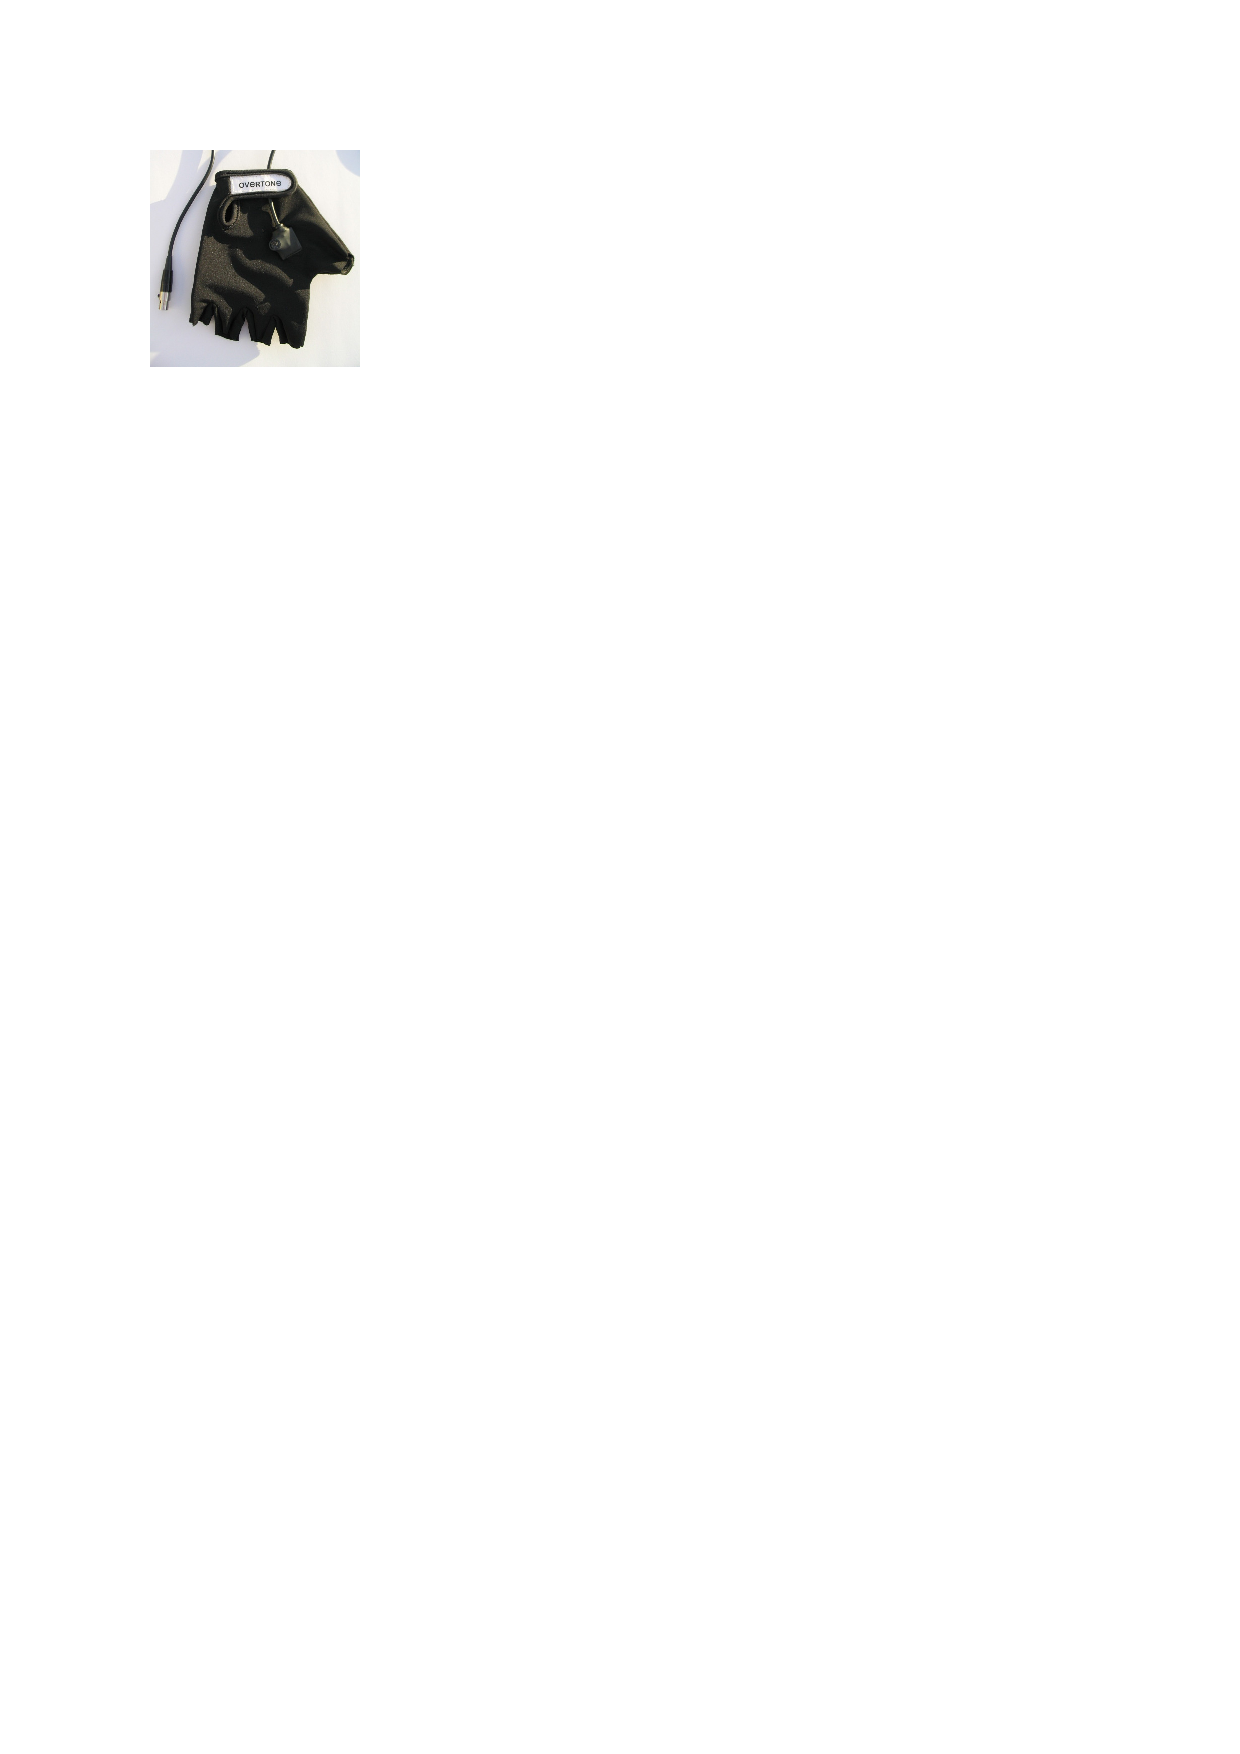
\includegraphics[height=45mm]{img-6-eps-converted-to.pdf}
\caption{The USB RF receiver and glove with sensors.}
\label{Overholt:fig:4} 
\end{figure}

The top side of the head of the violin includes the miniature video camera, the
16-button matrix, and one of the ultrasonic sonar sensors. The video camera can
of course provide content to be manipulated in a multi-media performance setting,
but this was only one of the reasons it was included with the sensors. One
gestural attribute that is unexploited in normal violin technique is the
direction the violin is pointing---the video camera (as well as the sonar) are
included for this reason, in order to capture information about whatever the
violin is pointing at. This can then be analyzed in the computer and used to
control different aspects of the sound. The sonar sensor determines the distance
from the end of the violin to any solid object such as a person or a wall; it
does this by sending out 40kHz bursts controlled by the PIC16F877 and waiting for
the echo to return once the signal has bounced off something. It calculates the
distance based on the speed of sound, and has a range of about 10 feet.

The back side of the head of the violin has one spring-loaded slider, a
miniature joystick, two linear potentiometers, and two buttons. All of these can
be thumb-controlled, except for the two buttons that are mounted in such a way
that they are accessible with the knuckles while playing the violin
strings---these are useful for changing modes without having to switch hand
positions. Any sensor may be assigned to any parameter on the computer of course,
but they are interconnected such that the left linear potentiometer controls an
offset for the spring-loaded slider, and the right linear potentiometer changes
the scaling factor for both axes of the joystick. This does not preclude using
either of the linear potentiometers independently, but it does allow the
sensitivity of the joystick to be fine-tuned, and the base level of the
spring-loaded slider to be set so that it doesn't always go all the way back to
zero; these interdependencies can be very useful while performing.

The Overtone Violin is played with a normal violin bow, as the performer wears a
glove with embedded gesture sensors (see Figure~\ref{Overholt:fig:4}) on the right hand. This glove
connects to the violin via a 5-pin mini-XLR jack located on the right side of the
body of the instrument. It is actually a fingerless nylon biking glove with a
small circuit board sewn on consisting of an accelerometer and a sonar
transducer. The accelerometer is an Analog Devices ADXL-203, which can sense both
acceleration and tilt (with respect to gravity) on two axes. This gives the
performer a virtual x/y joystick and captures relative gestures of the bowing
hand / arm. The sonar transducer is used to capture absolute movements between
the glove and the body of the violin. Like the sonar sensor on the head of the
violin, the glove sonar senses distance but it is set up for direct instead of
echo (reflection) mode. It has a range of 3 feet, corresponding roughly to the
distance from the glove to the violin when the right arm is fully extended. The
ultrasonic pulse is sent out from the glove transducer, and there are three
receiving transducers mounted on the body of the violin (just behind the string
support) in order to widen the angle of reception. The glove sensors provide the
performer with a set of gestures that are similar to bowing, yet can be used in a
completely different way (even without holding the bow). The performance
technique employed while using the gesture glove is actually more in the vein of
Michel Waisvisz's Hands \cite{Waisvisz:1985} than traditional violin practice. This is the main
reason the sensors were put into a glove instead of being attached to the bow,
but they can in fact be used as an approximation of bowing gestures while playing
on the strings if so desired.

\section{Conclusion}

The Overtone Violin\footnote{Video clips of the Overtone Violin can be found at the following web page:
\url{http://homes.create.aau.dk/dano/violin/}. The Overtone Violin is Patent Pending 2004.}
 is an ongoing project that will keep evolving. While this
paper outlines the technical development of the violin itself, current research
has focused on the development of new performance practices with it. The first
public performance with the Overtone Violin was at the Dutch Electronic Art
Festival (DEAF '04) in Rotterdam, the Netherlands.  The composition \textit{Duet
for Violin + Violinist} uses the SuperCollider 3 audio synthesis language to
process sounds from the violin strings as well as generate completely new sounds
through a mixture of different synthesis algorithms. It was inspired by the idea
of creating an improvisation environment with oneself, and trying to get away
from the division between accompanist and soloist. The Overtone Violin represents
a significant step towards formulating an integrated approach to new violin
performance; given the versatility and expressive performance possibilities of
the instrument, it is impossible to foresee the far-reaching effects it may have
on violin performance and composition.


\begin{acknowledgement}
Many thanks to Curtis Roads, JoAnn Kuchera-Morin, Stephen Pope, Keith Frezon,
Michel Waisvisz, Daniel Schorno, Rene Wassenburg, Wesley Brandt, and Anne-Marie
Skriver for all of their help and support.
\end{acknowledgement}

\section*{Author Commentary: Reflections on the Overtone Violin and Continuing Related Works}
\paragraph{Dan Overholt}

As a composer, improviser, inventor and instrument builder, I've been performing internationally with new musical instruments and custom sound synthesis and processing algorithms for quite a few years. I have used the Overtone Violin in both solo and collaborative works which have been included in major events such as the Spark Festival of Electronic Music and Arts, Woodstockhausen Festival of Electronic Music, the International Computer Music Conference (ICMC), the New Interfaces for Musical Expression Conference (NIME), U.C. San Diego's Center for Research in Computing and the Arts (CRCA), the Studio for Electro-Instrumental Music (STEIM), and the Dutch Electronic Art Festival (DEAF).

A large part of my development efforts for the Overtone Violin were funded through a Fulbright scholarship I took to STEIM in Amsterdam during 2003-04, and a National Science Foundation fellowship for research in Interactive Digital Multimedia at University of California, Santa Barbara from 2005-07. Both of these were during my time as a Ph.D. student in the Media Arts and Technology program at UCSB, under the guidance of Professor Curtis Roads. Follow-up research on the development of related instruments has more recently taken me to Stanford?s University's Center for Computer Research in Music and Acoustics (CCRMA) in 2010, via an H- STAR grant for research investigating actuated musical instruments \cite{Overholt:2011}.

While my skills as a luthier were definitely challenged during the building of the resulting Overtone Fiddle \cite{Overholt:2011a} (a semi-acoustic instrument, whereas the Overtone Violin is entirely solid-body electric), an actuator placed inside the body of the Fiddle allows more intimate playing experiences, because all sounds---processed or not---come from the body of the instrument. It can be played like a regular violin when not turned on, but signals that have been processed can also be put directly into the instrument?s body, causing it to resonate and produce a wider variety of sounds. An iPod Touch controls the signals, allowing the performer to modify effects on the fly, while a bow fitted with a position sensor provides another form of input that can be used to modify the sounds in a manner similar to the Overtone Violin. This allows my personal repertoire of extended techniques (as developed for the Overtone Violin originally) to continue to be useful with the newer Overtone Fiddle. Both instruments are still useful, depending on the context of use.

Personally, many hours of enjoyable music making continue with these instruments, and I have attempted to encapsulate a bigger picture of this area of research in \cite{Overholt:2012} by outlining my own classifications of related work. Also, and most recently, I have attempted to bring the cost and ease of replication of such instruments down to a more palatable level for every-day musicians. This has resulted in the creation of an accessible hybrid violin platform \cite{Overholt:2014}, the development of which was in part funded by the C.W. Obel foundation. In such manners, I hope to spread some of the immense pleasure I've gotten from the process of building and playing augmented instruments with a wider array of people around the world.

\section*{Expert Commentary: Augmenting instruments and extending cultures: on the Overtone Violin}
\paragraph{Federico Visi}

Dan Overholt's \textit{Overtone Violin} is a valuable contribution to the prolific branch of augmented instruments (also known as \textit{hyperinstruments}) that has been a part of NIME since its inception. As the author notes, instrument augmentation differs from the design of entirely novel digital musical interfaces as it relies on the extension and modification of relatively well-known instruments. This implies that the related techniques and repertoires play an important role in the design of an augmented instrument, since the designer often tries to build upon this pre-established knowledge. It is worth noting that the \textit{vocabulary of gestures} the author refers to not only allows musicians familiar with traditional violin techniques to easily approach the instrument. In fact, it also affects the experience of an audience attending a performance, given that the shared knowledge of said vocabulary of actions and movements influences the musical experience and it is also part of the embodied knowledge of individuals with no experience in playing the instrument \cite{Visi:2015}.

The approach adopted by Overholt aims at acknowledging the existing traditional techniques. At the same time, the addition of various sensors to control software parameters through movement requires the player to extend his or her technique. This approach also inherently addresses issues of expressivity, audience engagement and transparency of a performance with digital musical instruments. The `new vocabulary' that players are asked to learn is built upon (and to a certain extent constrained to) the violin idiom, and this dependency also affects the interaction with software through the motion sensors.

Parameter mapping has in fact been a debated topic since the early years of NIME \cite{Hunt:2002}. However, in later NIME conferences, the issue has shifted towards more conceptual territories where the instrument and the mapping that defines its use form an integral part of the musical composition \cite{Murray-Browne:2011}. The mapping strategies defining the digital component of the Overtone Violin are thus constrained by the fact that the instrument still \textit{is} a violin. Even though this may sound as a limitation at first, the affordances embedded in the genes of the instrument are, on the contrary, a cognitive resource for performers, composers and audiences alike. The virtually unlimited freedom that digital musical instruments offer will eventually be considered problematic for attaining a transparent and expressive performance as ``it is exactly this freedom of mapping that may disturb the sense of contact and of non-mediation'' \cite{Leman:2007}.

Traditional musical instruments are artefacts that carry a great deal of culture and shared knowledge in them. Designing an augmented violin is therefore not only a work of engineering but also a way of extending a layered cultural discourse with new gestures and behaviours. From this perspective, instrument augmentation is something very akin to hackers culture, which is itself a constituent part of the NIME philosophy. Rethinking a violin means also hacking the semiotic memes, morphemes and kinemes of the traditional musical instruments narrative.

